% =============================================================================
% sections/project_budget.tex  -  Section 5: Project Budget
%
% SCORING: 0--27 pts
%   Budget structure (0-6 pts):
%     - Summary with expenditure status                     (0-1 pt)
%     - Source of financial support                         (0-1 pt)
%     - Rover major items with cost values                  (0-1 pt)
%     - Drone major items with cost values                  (0-1 pt)
%     - COTS vs. custom indication                          (0-1 pt)
%     - Non-engineering costs provided                      (0-1 pt)
%   Budget analysis (0-21 pts):
%     - Quality and granularity                             (0-13 pts)
%     - Budgetary prudence (custom-made, cost-effective)    (0-8 pts)
% =============================================================================

\section{Project Budget}
\label{sec:budget}

The project budget is derived directly from the rover and drone product trees (Section~3.1).

\subsection{Budget Summary}
\label{subsec:budget_summary}

\begin{longtable}{@{}p{6.2cm}p{2.2cm}p{2.2cm}p{2.9cm}@{}}
\caption{Budget summary}
\label{tab:budget_summary} \\

\toprule
\textbf{Category} & \centering\textbf{Budget [\$]} & \centering\textbf{Spent [\$]} & \centering\textbf{Remaining [\$]} \tabularnewline
\midrule
\endhead

Rover hardware (COTS + custom)            & \raggedleft 14100 & \raggedleft 3094 & \raggedleft 11006 \tabularnewline
Drone hardware                            & \raggedleft 1500  & \raggedleft 542  & \raggedleft 958 \tabularnewline
Component delivery                        & \raggedleft 1000  & \raggedleft 0    & \raggedleft 1000 \tabularnewline
Software / licences                       & \raggedleft 800   & \raggedleft 0    & \raggedleft 800 \tabularnewline
Manufacturing / machining                 & \raggedleft 800   & \raggedleft 0    & \raggedleft 800 \tabularnewline
Operational and logistics costs           & \raggedleft 5000  & \raggedleft 0    & \raggedleft 5000 \tabularnewline
Spare parts and future upgrades           & \raggedleft 6800  & \raggedleft 0    & \raggedleft 6800 \tabularnewline
Risk and contingency reserve              & \raggedleft 5000  & \raggedleft 0    & \raggedleft 5000 \tabularnewline
\midrule
\textbf{Total approved budget}            & \raggedleft\textbf{35000} & \raggedleft\textbf{3636} & \raggedleft\textbf{31364} \tabularnewline
\bottomrule
\end{longtable}

The budget includes reserves for manufacturing, logistics, spare parts, and contingency,
ensuring financial robustness during integration and testing.

\begin{figure}[H]
\centering
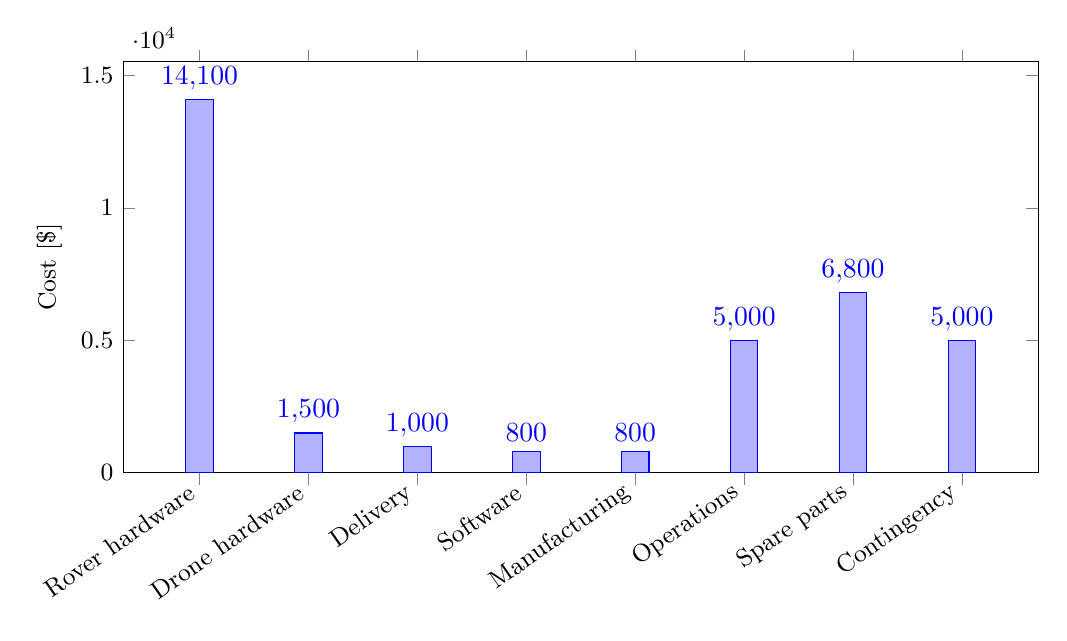
\begin{tikzpicture}
\begin{axis}[
    width=13.2cm,
    height=6.8cm,
    ybar,
    bar width=10pt,
    ymin=0,
    ylabel={Cost [\$]},
    symbolic x coords={
        Rover hardware,
        Drone hardware,
        Delivery,
        Software,
        Manufacturing,
        Operations,
        Spare parts,
        Contingency
    },
    xtick=data,
    x tick label style={rotate=35, anchor=east, font=\small},
    ylabel style={font=\small},
    tick label style={font=\small},
    nodes near coords,
    nodes near coords align={vertical}
]
\addplot coordinates {
    (Rover hardware,14100)
    (Drone hardware,1500)
    (Delivery,1000)
    (Software,800)
    (Manufacturing,800)
    (Operations,5000)
    (Spare parts,6800)
    (Contingency,5000)
};
\end{axis}
\end{tikzpicture}
\caption{Distribution of the total approved project budget.}
\label{fig:budget_distribution}
\end{figure}

Figure~\ref{fig:budget_distribution} shows that the largest budget share is allocated to rover hardware,
operations, spare parts, and contingency, reflecting system complexity and risk mitigation needs.

\begin{longtable}{@{}p{5.5cm}p{2.2cm}p{5.8cm}@{}}
\caption{Sources of financial support}
\label{tab:budget_sources} \\

\toprule
\textbf{Source} & \centering\textbf{Amount (\$)} & \textbf{Notes} \tabularnewline
\midrule
\endfirsthead

\toprule
\textbf{Source} & \centering\textbf{Amount (\$)} & \textbf{Notes} \tabularnewline
\midrule
\endhead

Ukrainian Catholic University & \raggedleft 35000 & supported by Nova Ukraine, SoftServe, ELEKS, and Infineon \tabularnewline

\midrule
\textbf{Total} & \raggedleft\textbf{35000} & \tabularnewline
\bottomrule
\end{longtable}

\subsection{Budget Table Based on Product Tree}
\label{subsec:budget_product_tree}

Table~\ref{tab:product_tree_budget} presents the major hardware items derived from the product tree,
serving as the primary link between system architecture and budget allocation.

{\small
\begin{longtable}{@{}p{0.7cm}p{1.8cm}p{2.5cm}p{4.2cm}p{1.1cm}p{0.9cm}p{1.3cm}@{}}
\caption{Project budget based on the product tree}
\label{tab:product_tree_budget} \\

\toprule
\textbf{No.} &
\textbf{High Level} &
\textbf{Low Level} &
\textbf{Part or minor assembly / subassembly} &
\centering\textbf{Price} &
\centering\textbf{Qty} &
\centering\textbf{Total} \tabularnewline
&
\textbf{Subsystem Name} &
\textbf{Subsystem} &
&
\centering\textbf{[\$]} &
&
\centering\textbf{[\$]} \tabularnewline
\midrule
\endfirsthead

\toprule
\textbf{No.} &
\textbf{High Level} &
\textbf{Low Level} &
\textbf{Part or minor assembly / subassembly} &
\centering\textbf{Price} &
\centering\textbf{Qty} &
\centering\textbf{Total} \tabularnewline
&
\textbf{Subsystem Name} &
\textbf{Subsystem} &
&
\centering\textbf{[\$]} &
&
\centering\textbf{[\$]} \tabularnewline
\midrule
\endhead

1  & Rover & Operation and control & Main computer --- NVIDIA Jetson Orin NX 16GB & \raggedleft 1048 & \centering 1 & \raggedleft 1048 \tabularnewline
2  & Rover & Operation and control / Video subsystem & Nav camera --- ArduCam AR0234 & \raggedleft 155 & \centering 2 & \raggedleft 310 \tabularnewline
3  & Rover & Operation and control / Video subsystem & Main nav camera --- ArduCam Stereo AR0234 & \raggedleft 260 & \centering 1 & \raggedleft 260 \tabularnewline
4  & Rover & Operation and control / Communication subsystem & Wi-Fi adapter (mast) --- Alfa AWUS036ACH & \raggedleft 100 & \centering 1 & \raggedleft 100 \tabularnewline
5  & Rover & Chassis / Body & Body structure & \raggedleft 200 & \centering 1 & \raggedleft 200 \tabularnewline
6  & Rover & Chassis / Drive module & Drive motor --- DM-J10010L & \raggedleft 221 & \centering 4 & \raggedleft 884 \tabularnewline
7  & Rover & Chassis / Drive module & Rotation motor --- DM-J4340 & \raggedleft 260 & \centering 4 & \raggedleft 1040 \tabularnewline
8  & Rover & Power module & Batteries + BMS --- 48V 12Ah battery & \raggedleft 160 & \centering 4 & \raggedleft 640 \tabularnewline
9  & Rover & Arm / Base & High-torque planetary actuator --- SteadyWin GIM8115-36 & \raggedleft 260 & \centering 3 & \raggedleft 780 \tabularnewline
10 & Rover & Arm / Manipulation & Low-torque planetary actuator --- DAMIAO DM-J4340-2EC & \raggedleft 170 & \centering 3 & \raggedleft 510 \tabularnewline
11 & Rover & Arm & Arm controller --- Raspberry Pi 4 (8GB RAM) & \raggedleft 110 & \centering 1 & \raggedleft 110 \tabularnewline
12 & Rover & Arm & Arm camera --- ArduCam AR0234 USB 3.0 & \raggedleft 125 & \centering 1 & \raggedleft 125 \tabularnewline
13 & Rover & Science / Exploration system & Spectral camera --- MAPIR Survey3W OCN & \raggedleft 500 & \centering 1 & \raggedleft 500 \tabularnewline
14 & Rover & Science / Exploration system & Thermal camera --- CADDX FPV ECLIPSE 640SH + Caddx Avatar GT VTX & \raggedleft 200 & \centering 1 & \raggedleft 200 \tabularnewline
15 & Rover & Science / Sample collection gripper & Drill motor --- DC RS-775SH & \raggedleft 50 & \centering 1 & \raggedleft 50 \tabularnewline
16 & Rover & Science / Sample collection gripper & Drill driver --- BTS7960 H-bridge & \raggedleft 20 & \centering 1 & \raggedleft 20 \tabularnewline
17 & Rover & Science / Liquid analysis system & pH-sensor --- Grove pH Sensor E-201C-Blue & \raggedleft 30 & \centering 1 & \raggedleft 30 \tabularnewline
18 & Rover & Science / Liquid analysis system & Liquid pump system & \raggedleft 20 & \centering 1 & \raggedleft 20 \tabularnewline
19 & Rover & Navigation & LiDAR --- RPLIDAR S2 & \raggedleft 266 & \centering 1 & \raggedleft 266 \tabularnewline
20 & Rover & Navigation & ToF camera --- Maix Sense A010 ToF & \raggedleft 120 & \centering 1 & \raggedleft 120 \tabularnewline
21 & Rover & Navigation & Human presence sensor --- HLK-LD2450 Human Tracking Radar & \raggedleft 50 & \centering 1 & \raggedleft 50 \tabularnewline
22 & Drone & Control & Flight controller --- Pixhawk 6C & \raggedleft 138 & \centering 1 & \raggedleft 138 \tabularnewline
23 & Drone & Control & Companion computer --- Raspberry Pi 5 (16GB RAM) & \raggedleft 180 & \centering 1 & \raggedleft 180 \tabularnewline
24 & Drone & Perception & GPS \& Compass module --- Holybro M10 GPS Module & \raggedleft 60 & \centering 1 & \raggedleft 60 \tabularnewline
25 & Drone & Perception & Optical flow sensor --- MicroAir MTF-01 & \raggedleft 50 & \centering 1 & \raggedleft 50 \tabularnewline
26 & Drone & Perception & Forward camera --- Foxeer Cat4 & \raggedleft 40 & \centering 1 & \raggedleft 40 \tabularnewline
27 & Drone & Communication & ELRS receiver --- RP1 V2 ExpressLRS 2.4GHz Nano Receiver & \raggedleft 17 & \centering 1 & \raggedleft 17 \tabularnewline
28 & Drone & Communication & RC controller / ELRS transmitter --- TX16S & \raggedleft 260 & \centering 1 & \raggedleft 260 \tabularnewline
29 & Drone & Power & LiPo battery --- Turnigy 5000mAh 5S 30C Lipo Pack & \raggedleft 60 & \centering 1 & \raggedleft 60 \tabularnewline
30 & Drone & Propulsion & ESC --- Brushless 30A ESC & \raggedleft 15 & \centering 4 & \raggedleft 60 \tabularnewline
31 & Drone & Propulsion & Motors --- 2212/920KV DJI brushless motors & \raggedleft 10 & \centering 4 & \raggedleft 40 \tabularnewline
32 & Travel & Transport & Transport to competition & \raggedleft 951 & \centering 1 & \raggedleft 951 \tabularnewline
33 & Travel & Accommodation & Accommodation during competition & \raggedleft 1729 & \centering 1 & \raggedleft 1729 \tabularnewline
34 & Travel & Food & Team meals & \raggedleft 1038 & \centering 1 & \raggedleft 1038 \tabularnewline
35 & Travel & Logistics & Ground station miscellaneous / logistics & \raggedleft 300 & \centering 1 & \raggedleft 300 \tabularnewline

\midrule
\textbf{Total 1} & \textbf{Rover} & & & & & \raggedleft\textbf{7263} \tabularnewline
\textbf{Total 2} & \textbf{Drone} & & & & & \raggedleft\textbf{905} \tabularnewline
\textbf{Total 3} & \textbf{Other costs} & & & & & \raggedleft\textbf{4018} \tabularnewline
\textbf{Total 4} & \textbf{All above} & & & & & \raggedleft\textbf{12186} \tabularnewline
\bottomrule
\end{longtable}
}

The product-tree baseline amounts to 12\,186~\$, including 7\,263~\$ (rover), 905~\$ (drone),
and 4\,018~\$ (non-engineering costs). The remaining budget is reserved for custom components,
integration, software, spare parts, and contingency.

\begin{figure}[H]
\centering
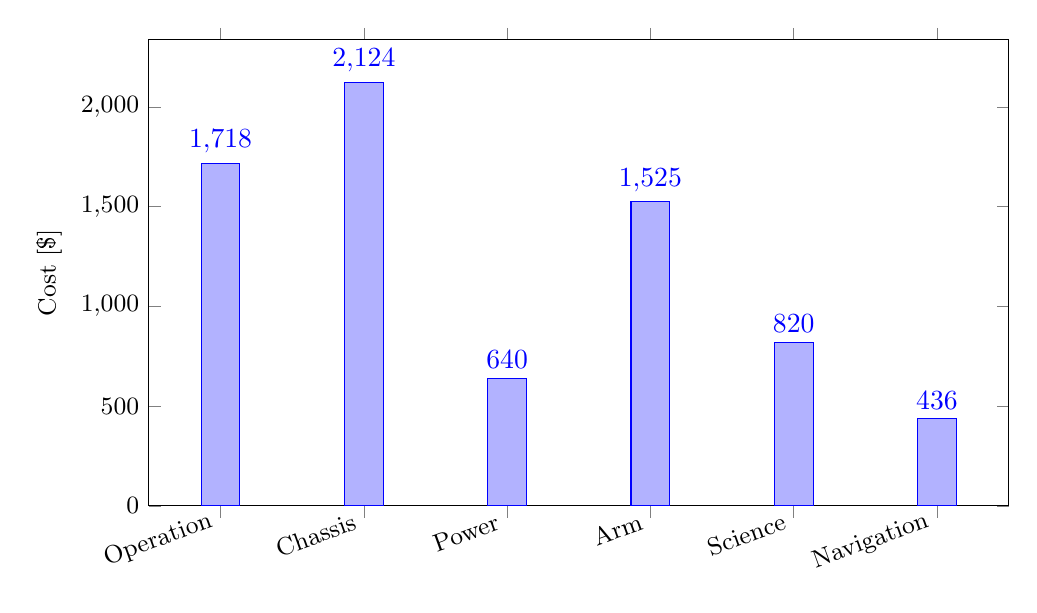
\begin{tikzpicture}
\begin{axis}[
    width=12.5cm,
    height=7.5cm,
    ybar,
    bar width=14pt,
    ymin=0,
    ylabel={Cost [\$]},
    symbolic x coords={
        Operation,
        Chassis,
        Power,
        Arm,
        Science,
        Navigation
    },
    xtick=data,
    x tick label style={rotate=20, anchor=east, font=\small},
    ylabel style={font=\small},
    tick label style={font=\small},
    nodes near coords,
    nodes near coords align={vertical}
]
\addplot coordinates {
    (Operation,1718)
    (Chassis,2124)
    (Power,640)
    (Arm,1525)
    (Science,820)
    (Navigation,436)
};
\end{axis}
\end{tikzpicture}
\caption{Rover hardware cost distribution by subsystem, derived from the product-tree budget table.}
\label{fig:rover_subsystem_costs}
\end{figure}

Figure~\ref{fig:rover_subsystem_costs} shows that the main rover cost drivers are the chassis,
operation and control, and manipulator subsystems.

\subsection{COTS and Custom Components}
\label{subsec:cots_custom}

The design uses a mixed COTS and custom approach. COTS components are selected for critical subsystems
to ensure reliability and fast integration, while custom parts are limited to structural elements required
by the rover geometry.

{\small
\begin{longtable}{@{}p{7.2cm}p{4.0cm}p{2.0cm}@{}}
\caption{Rover custom-manufactured components}
\label{tab:rover_custom} \\

\toprule
\textbf{Component} & \textbf{Subsystem} & \centering\textbf{Cost (\$)} \tabularnewline
\midrule
\endfirsthead

\toprule
\textbf{Component} & \textbf{Subsystem} & \centering\textbf{Cost (\$)} \tabularnewline
\midrule
\endhead

TPU 3D-printed parts & Chassis / Arm / Science & \raggedleft 1000 \tabularnewline
Machining and fabrication of metal parts & Chassis / Structure & \raggedleft 800 \tabularnewline
Custom carriage / integration assemblies & Mobility & \raggedleft 500 \tabularnewline

\midrule
\textbf{Custom subtotal} & & \raggedleft\textbf{2300} \tabularnewline
\bottomrule
\end{longtable}
}

\begin{longtable}{@{}p{6cm}p{3cm}@{}}
\caption{Cost distribution between COTS and custom rover components}
\label{tab:rover_cots_custom} \\

\toprule
\textbf{Type} & \centering\textbf{Cost (\$)} \tabularnewline
\midrule
\endfirsthead

\toprule
\textbf{Type} & \centering\textbf{Cost (\$)} \tabularnewline
\midrule
\endhead

COTS rover components & \raggedleft 11800 \tabularnewline
Custom rover components & \raggedleft 2300 \tabularnewline

\midrule
\textbf{Total rover hardware} & \raggedleft\textbf{14100} \tabularnewline
\bottomrule
\end{longtable}

The drone is designed as an almost fully COTS subsystem. This reduces manufacturing effort and integration
risk while maintaining adequate functionality for auxiliary mission tasks.

\subsection{Non-Engineering Costs}
\label{subsec:non_engineering_costs}

{\small
\begin{longtable}{@{}p{5.8cm}p{1.5cm}p{6.0cm}@{}}
\caption{Operational and logistics costs}
\label{tab:operational_costs} \\

\toprule
\textbf{Item} & \centering\textbf{Cost (\$)} & \textbf{Notes} \tabularnewline
\midrule
\endfirsthead

\toprule
\textbf{Item} & \centering\textbf{Cost (\$)} & \textbf{Notes} \tabularnewline
\midrule
\endhead

Accommodation & \raggedleft 1729 & team stay during competition \tabularnewline
Travel to competition & \raggedleft 951 & transport to Poland \tabularnewline
Food & \raggedleft 1038 & team meals during competition \tabularnewline
Rover transportation & \raggedleft 26 & rover transport logistics \tabularnewline
Return travel & \raggedleft 778 & transport back after competition \tabularnewline
Local transportation and logistics & \raggedleft 250 & local mobility, fuel, transfers \tabularnewline
Equipment handling and packing & \raggedleft 228 & packaging, tools, consumables \tabularnewline

\midrule
\textbf{Total operational costs} & \raggedleft\textbf{5000} & \tabularnewline
\bottomrule
\end{longtable}
}

\begin{longtable}{@{}p{6cm}p{3cm}@{}}
\caption{Delivery costs for hardware procurement}
\label{tab:delivery_costs} \\

\toprule
\textbf{Category} & \centering\textbf{Cost (\$)} \tabularnewline
\midrule
\endfirsthead

\toprule
\textbf{Category} & \centering\textbf{Cost (\$)} \tabularnewline
\midrule
\endhead

International shipping of electronics and sensors & \raggedleft 635 \tabularnewline
Local delivery of mechanical parts and materials & \raggedleft 250 \tabularnewline
Additional shipping overhead and contingencies & \raggedleft 115 \tabularnewline

\midrule
\textbf{Total delivery} & \raggedleft\textbf{1000} \tabularnewline
\bottomrule
\end{longtable}

\subsection{Budget Analysis}
\label{subsec:budget_analysis}

The budget reflects the system architecture, with the rover accounting for the largest share due to its
mechanical complexity, sensing requirements, and integration effort. The main cost drivers are actuators,
onboard computing, and the mobility system.

A mixed COTS and custom strategy is applied. COTS components are used for high-risk and time-critical
functions (computing, sensing, communication), ensuring reliability and faster integration. Custom
manufacturing is limited to structural and integration elements, where it is more cost-effective.

The drone is designed as a low-cost, mostly COTS subsystem, minimizing development effort while preserving
functionality. Non-engineering costs are separated for transparency. The remaining budget is reserved for
integration, spare parts, and contingency, ensuring robustness during testing and deployment.
